%! TEX program = lualatex
%! TEX root = defense.tex
\documentclass[professionalfont,fleqn]{beamer}

\usepackage{polyglossia}
\setdefaultlanguage[variant=us]{english}
\usepackage{array}
\usepackage{amsmath}
\usepackage{booktabs}
\usepackage{csquotes}
\usepackage{grfext}
\usepackage{listings}
\usepackage{multirow}
\usepackage{pgfpages}
\usepackage{pgfplots}
\usepackage{pgfplotstable}
\usepackage{pgf-pie}
\usepackage{pbox}
\usepackage[mode=text,binary-units,separate-uncertainty=true,multi-part-units=single]{siunitx}
% \usepackage[caption=false]{subfig}
\usepackage{tikz}
\usepackage[compat=1.1.0]{tikz-feynman}
\usepackage{threeparttablex}
\usepackage{tabularx}
\usepackage{textpos}
\usepackage{unicode-math}
\usepackage{xpatch}
\usepackage{xspace}
\usepackage{xcolor}
\usepackage{xstring}
\usepackage[makeroom]{cancel}
\usepackage{appendixnumberbeamer}

\pgfplotsset{compat=1.14}

\usetikzlibrary{fit,backgrounds,calc,matrix,scopes,shapes.arrows}

\lstMakeShortInline|

\PrependGraphicsExtensions*{.pdf,.PDF}

\DeclareDocumentCommand\Pe{}{\ensuremath{e}\xspace}
\DeclareDocumentCommand\Pgamma{}{\ensuremath{γ}\xspace}
\DeclareDocumentCommand\Pnu{}{\ensuremath{ν}\xspace}
\DeclareDocumentCommand\Pmu{}{\ensuremath{μ}\xspace}
\DeclareDocumentCommand\Ptop{}{\ensuremath{\text{t}}\xspace}
\DeclareDocumentCommand\Pu{}{\ensuremath{u}\xspace}
\DeclareDocumentCommand\Pd{}{\ensuremath{d}\xspace}
\DeclareDocumentCommand\Pc{}{\ensuremath{c}\xspace}
\DeclareDocumentCommand\Ps{}{\ensuremath{s}\xspace}
\DeclareDocumentCommand\Pb{}{\ensuremath{\text{b}}\xspace}
\DeclareDocumentCommand\Pq{}{\ensuremath{\text{q}}\xspace}
\DeclareDocumentCommand\Pj{}{\ensuremath{\text{j}}\xspace}
\DeclareDocumentCommand\PW{}{\ensuremath{\text{W}}\xspace}
\DeclareDocumentCommand\PH{}{\ensuremath{\text{H}}\xspace}
\DeclareDocumentCommand\PZ{}{\ensuremath{\text{Z}}\xspace}
\DeclareDocumentCommand\Pg{}{\ensuremath{\text{g}}\xspace}
\DeclareDocumentCommand\Phad{}{\ensuremath{h}\xspace}
\DeclareDocumentCommand\Plep{}{\ensuremath{ℓ}\xspace}
\DeclareDocumentCommand\Ptauh{}{\ensuremath{{\Ptau_\Phad}}\xspace}
\DeclareDocumentCommand\Ppi{}{\ensuremath{π}\xspace}
\DeclareDocumentCommand\Ppizero{}{\ensuremath{π^0}\xspace}
\DeclareDocumentCommand\Ppiplus{}{\ensuremath{π^+}\xspace}
\DeclareDocumentCommand\Ppiminus{}{\ensuremath{π^-}\xspace}
\DeclareDocumentCommand\Pkaon{}{\ensuremath{K}\xspace}
\DeclareDocumentCommand\Prho{}{\ensuremath{ρ}\xspace}

\DeclareDocumentCommand\pTmiss{}{\ensuremath{\pT^\text{miss}}\xspace}
\DeclareDocumentCommand\Pbb{}{\ensuremath{\Pb\bar{\Pb}}\xspace}
\DeclareDocumentCommand\PWW{}{\ensuremath{\PW\PW}\xspace}
\DeclareDocumentCommand\Ptautau{}{\ensuremath{\Ptau\Ptau}\xspace}
\DeclareDocumentCommand\Ptt{}{\ensuremath{\Ptop\bar{\Ptop}}\xspace}
\DeclareDocumentCommand\PttH{}{\ensuremath{\Ptop\bar{\Ptop}\PH}\xspace}
\DeclareDocumentCommand\PttZ{}{\ensuremath{\Ptop\bar{\Ptop}\PZ}\xspace}
\DeclareDocumentCommand\PttW{}{\ensuremath{\Ptop\bar{\Ptop}\PW}\xspace}
\DeclareDocumentCommand\PWjets{}{\ensuremath{\PW+\text{jets}}\xspace}
\DeclareDocumentCommand\PZZ{}{\ensuremath{\PZ\PZ}\xspace}

\DeclareDocumentCommand\pT{}{\ensuremath{p_\text{T}}\xspace}

\DeclareDocumentCommand\lumi{}{\SI{35.9}{\per\femto\barn}\xspace}
\DeclareDocumentCommand\ttH{}{\ensuremath{\Ptop\bar{\Ptop}\PH}\xspace}
\DeclareDocumentCommand\ttZ{}{\ensuremath{\Ptop\bar{\Ptop}\PZ}\xspace}
\DeclareDocumentCommand\ttW{}{\ensuremath{\Ptop\bar{\Ptop}\PW}\xspace}
\DeclareDocumentCommand\ttbar{}{\ensuremath{\Ptop\bar{\Ptop}}\xspace}
\DeclareDocumentCommand\qqbar{}{\ensuremath{\Pq\Pqbar}\xspace}
\DeclareDocumentCommand\bbbar{}{\ensuremath{\text{b}\bar{\text{b}}}\xspace}
\DeclareDocumentCommand\ccbar{}{\ensuremath{\text{b}\bar{\text{b}}}\xspace}
\DeclareDocumentCommand\ttX{}{\ensuremath{\Ptop(\bar{\Ptop})\text{X}}\xspace}
\newcommand{\ttV}{\ensuremath{t\overline{t}V}\xspace}

\DeclareDocumentCommand\cB{}{\ensuremath{\bar{c}_{\text{B}}}\xspace}
\DeclareDocumentCommand\cH{}{\ensuremath{\bar{c}_{\text{H}}}\xspace}
\DeclareDocumentCommand\cHB{}{\ensuremath{\bar{c}_{\text{HB}}}\xspace}
\DeclareDocumentCommand\cHu{}{\ensuremath{\bar{c}_{\text{Hu}}}\xspace}
\DeclareDocumentCommand\cHud{}{\ensuremath{\bar{c}_{\text{Hud}}}\xspace}
\DeclareDocumentCommand\cHQ{}{\ensuremath{\bar{c}_{\text{HQ}}}\xspace}
\DeclareDocumentCommand\cpHQ{}{\ensuremath{\bar{c}^{\prime}_{\text{HQ}}}\xspace}
\DeclareDocumentCommand\cthreeG{}{\ensuremath{\bar{c}_{\text{3G}}}\xspace}
\DeclareDocumentCommand\cthreeW{}{\ensuremath{\bar{c}_{\text{3W}}}\xspace}
\DeclareDocumentCommand\ctwoG{}{\ensuremath{\bar{c}_{\text{2G}}}\xspace}
\DeclareDocumentCommand\cu{}{\ensuremath{\bar{c}_\text{u}}\xspace}
\DeclareDocumentCommand\cuB{}{\ensuremath{\bar{c}_{\text{uB}}}\xspace}
\DeclareDocumentCommand\cuG{}{\ensuremath{\bar{c}_{\text{uG}}}\xspace}
\DeclareDocumentCommand\cuW{}{\ensuremath{\bar{c}_{\text{uW}}}\xspace}
\DeclareDocumentCommand\tcA{}{\ensuremath{\widetilde{c}_{\text{A}}}\xspace}
\DeclareDocumentCommand\tcHW{}{\ensuremath{\widetilde{c}_{\text{HW}}}\xspace}
\DeclareDocumentCommand\tcthreeG{}{\ensuremath{\widetilde{c}_{\text{3G}}}\xspace}

\usepackage{mathtools}
\DeclarePairedDelimiter{\abs}{\lvert}{\rvert}

\tikzset{
  rot/.style={rotate=90},
  tiny/.style={font=\tiny},
  ndbox/.style={rounded corners,fill=yellow,text=blue}}

\lstset{
  basicstyle=\ttfamily,
  breaklines=true,
  breakindent=2ex}

\usetheme[sectionpage=simple,numbering=fraction]{metropolis}
\setbeamerfont{section in toc}{size=\large,shape=\bfseries}

\AtBeginSection[]
{
  \begingroup
  \renewcommand{\insertframenumberfraction}{}
  \begin{frame}[noframenumbering]{Outline}
    \begin{center}
      \tableofcontents[currentsection]
    \end{center}
  \end{frame}
  \endgroup
}

\author{Anna Woodard}
\date{February 27, 2018}
\title{Effective field theory interpretation for measurements of top quark
pair-production in association with a W or Z boson}
\subtitle{Dissertation Defense}

\definecolor{purple}{HTML}{bf80ff}

\newcolumntype{C}[1]{ >{\centering\arraybackslash} m{#1} }
\newcolumntype{L}[1]{>{\raggedright\let\newline\\\arraybackslash\hspace{0pt}}m{#1}}

\begin{document}

\pgfdeclarelayer{foreground}
\pgfdeclarelayer{background}
\pgfsetlayers{background,main,foreground}

\maketitle

\begin{frame}{The Large Hadron Collider (LHC)}
  \begin{columns}
    \begin{column}{.4\linewidth}
      \centering
      \includegraphics[width=5cm]{figures/LHC}
    \end{column}
    \begin{column}{.6\linewidth}
      \small
      \begin{itemize}
        \item \SI{26.7}{km} tunnel
        \item \SI{8}{TeV} center-of-mass energy, upgraded to \SI{13}{TeV} starting in 2015 (\SI{3.1}{m/s} slower than light)
        \item Superconducting magnet temperature is \SI{2}{K} (colder than outer space)
        % \item Total beam energy: \SI{260}{MJ} ($\approx$ kinetic energy of 750 Honda Civics each moving at \SI{55}{MPH})
        % \item Colliding protons is like shooting two needles at each other from a distance of six miles and having them hit in the middle
      \end{itemize}
    \end{column}
  \end{columns}
\end{frame}

\begin{frame}{The Large Hadron Collider (LHC)}
  \addtocounter{framenumber}{-1}
  \begin{columns}
    \begin{column}{.4\linewidth}
      \centering
      \includegraphics[width=5cm]{figures/LHC}
    \end{column}
    \begin{column}{.5\linewidth}

      \Huge
      \centering
    Why did we build the LHC?
    \end{column}
  \end{columns}
}
\end{frame}

\section{Theory}

\begin{frame}{The standard model (SM)}
  \begin{itemize}
    \item Basic idea
      \begin{itemize}
        \item Matter is made up of combinations of fundamental particles
          \begin{itemize}
            \item Fundamental particles are excitations of quantum fields
          \end{itemize}
        \item Particles interact via several forces
          \begin{itemize}
            \item Forces are associated with couplings between fermion `matter' fields and `boson' fields
          \end{itemize}
      \end{itemize}
  \end{itemize}
\end{frame}


\begin{frame}{The SM and beyond}
  \begin{columns}
    \begin{column}{.6\linewidth}
      \begin{figure}
    \includegraphics[width=7cm]{figures/sm}
      \end{figure}
    \end{column}
    \begin{column}{.4\linewidth}
      We know this picture is incomplete!
      \begin{itemize}
        \item Gravity
        \item Dark matter
        \item Dark energy
        \item etc etc
      \end{itemize}
    \end{column}
  \end{columns}
\end{frame}

\begin{frame}{Physics beyond the SM}
  \addtocounter{framenumber}{-1}
  \begin{columns}
    \begin{column}{.6\linewidth}
      \begin{figure}
        \includegraphics[width=7cm]{figures/sm-np}
      \end{figure}
    \end{column}
    \begin{column}{.4\linewidth}
      There must be particles we have not discovered yet!
    \end{column}
  \end{columns}
\end{frame}

\begin{frame}{How do we find new particles?}
  \centering
  Turn kinetic energy into mass!\\
  $E \Longleftrightarrow mc^2$\\
  \textcolor{red}{In red: particles discovered at particle accelerators of higher and higher energy}
  \includegraphics[width=11cm]{figures/particles}
\end{frame}

\begin{frame}[standout]
  Bad news: finding new particles may require more energy than the LHC provides
  \vspace{2cm}

  Good news: we have tools for coping; one is effective field theory (EFT)
\end{frame}

\begin{frame}{What is an effective theory?}
  \centering
  An effective theory describes observations without claiming that the mechanism of the theory is the actual cause of observations (expect a more fundamental underlying theory)
  % When we interpret things around us as made of solid matter, we are using an e ective theory. Ordinary matter is mostly empty space, but if we are building a table, it is not necessary to take that into account as we swing a hammer. Newtonian mechanics works extremely well, but it is an approximation for low speeds and large objects. Relativity and quantum mechanics are more fundamental underlying theories, but using relativity and quantum mechanics to calculate the trajectory of a cannon ball would be wasted e ort. 
  \begin{tabular}{lC{2.5cm}r}
    \parbox[c]{3cm}{\centering\includegraphics[width=3cm]{figures/table}\\`solid' matter} &
      
\begin{tikzpicture}
        \node[single arrow,fill=blue,minimum height=10mm,minimum width=10mm] {};
      \end{tikzpicture} &
    \parbox[c]{4cm}{\centering\includegraphics[width=2cm]{figures/atom}\\atomic theory} \\
    \parbox[c]{3cm}{\centering\includegraphics[width=3cm]{figures/newtonian}\\newtonian mechanics} &
      
\begin{tikzpicture}
        \node[single arrow,fill=blue,minimum height=10mm,minimum width=10mm] {};
      \end{tikzpicture} &
    \parbox[c]{4cm}{\centering\includegraphics[width=2cm]{figures/relativity}\\general relativity/\\quantum mechanics} \\
  \end{tabular}
\end{frame}

\begin{frame}{Effective field theory}
  Extend SM with higher dimensional operators representing new
physics associated with particles too heavy to produce at current collider energies

\begin{equation*}
  \mathcal{L}_{\textup{eff}} = \mathcal{L}^{(4)}_{\textup{SM}} + \underbrace{\xcancel{\frac{1}{\Lambda} c_1 \mathcal{O}_1^{(5)}}}_{\text{violates lep \#}}
  + \frac{1}{\Lambda^2} \sum_j c_j \mathcal{O}_j^{(6)} + ...
\end{equation*}
\textbf{Mass scale} of NP is $\Lambda$ (EFT valid for $E < \Lambda$)

\textbf{Operators} are all possible unique products of SM fields (which respect SM gauge symmetries), in this work focus on dimension six: $\mathcal{O}_j^{(6)}$

\textbf{Wilson coefficients} $c_j$ are dimensionless constants which characterize the strength of the NP effect (our goal: constrain these)

% TODO explain model independence
\end{frame}

\begin{frame}{Top quark physics}
  \vspace{2mm}
  \begin{columns}
    \begin{column}{.35\linewidth}
      Why study EFT in the top sector? Top's huge mass stands out--- is it special?
    \end{column}
    \begin{column}{.65\linewidth}
      \begin{tabular}{C{3cm}C{3.5cm}}
        % \multicolumn{2}{C{6.3cm}}{Top is so heavy that nothing decays to it: study associated production!}\\
        \textbf{Tops + Z (\ttZ)}&
        \only<1>{\resizebox{2.5cm}{!}{
\RequirePackage{luatex85}
\documentclass[tikz, border=10pt]{standalone}

\usepackage[compat=1.1.0]{tikz-feynman}

\newcommand{\Ptop}{\ensuremath{\text{t}}}

\makeatletter
\tikzset{
  position/.style args={#1 degrees from #2}{
    at=(#2.#1), anchor=#1+180, shift=(#1:\tikz@node@distance)
  }
}
\makeatother

\begin{document}

\tikzfeynmanset{
  proton/.style={
    draw=black,
    preaction={
      draw=black,
      double,
      double distance=3pt
    },
    /tikzfeynman/with arrow=0.5,
    % /tikz/postaction={
    %   /tikz/draw,
    %   /tikz/
    %   /tikzfeynman/with arrow=0.5
    % }
  }
}
\begin{tikzpicture}
  \begin{feynman}
    \diagram [horizontal'=hi to hf,tree layout,sibling distance=12mm,level distance=20mm] {
      % Higgs
      hi -- [draw=none] t1f,
      hi -- [scalar,edge label'=\(H\)] hf,
      hi -- [draw=none] t2f,
      % τ 1
      hf -- [fermion,edge label'=\(τ^-\)] t1
         -- [fermion] n1 [particle=\(\nu_\tau\)],
      t1 -- [boson,edge label=\(W^-\)] w1
         -- [fermion] f1 [particle=\(q\)],
      w1 -- [anti fermion] f2 [particle=\(\overline q'\)],
      % τ 2
      hf -- [anti fermion,edge label=\(τ^+\)] t2
         -- [boson,edge label'=\(W^+\)] w2
         -- [fermion] f3 [particle=\(q\)],
      w2 -- [anti fermion] f4 [particle=\(\overline q'\)],
      t2 -- [anti fermion] n2 [particle=\(\overline \nu_\tau\)],
      % top
      t1f -- [anti fermion] b1f [particle=\(\overline b\)],
      t1f -- [boson,edge label=\(W^-\)] w1f -- [anti fermion] j1 [particle=\(\overline q'\)],
      w1f -- [fermion] j2 [particle=\(q\)],
      % other top
      t2f -- [boson,edge label'=\(W^+\)] w2f -- [fermion] l2 [particle=\(\Pnu_\ell\)],
      t2f -- [fermion] b2f [particle=\(b\)],
      w2f -- [anti fermion] l1 [particle=\(\ell^+\)],
    };

    \vertex[above left=30mm and 6mm of hi] (t2i);
    \vertex[blob,above left=25mm and 20mm of t2i] (p2) {};
    \vertex[particle=\(p\),left=25mm of p2] (p2i) {\(p\)};
    \vertex[above right=5mm and 25mm of p2] (p2f);

    \vertex[below left=30mm and 6mm of hi] (t1i);
    \vertex[blob,below left=25mm and 20mm of t1i] (p1) {};
    \vertex[particle=\(p\),left=25mm of p1] (p1i) {\(p\)};
    \vertex[below right=5mm and 25mm of p1] (p1f);

    \diagram* {
      {[edges=proton]
        (p1i) [particle=\(p\)] -- (p1) [blob] -- (p1f),
        (p2i) [particle=\(p\)] -- (p2) [blob] -- (p2f),
      },
      (p1) [blob] -- [gluon,edge label=\(g\)] (t1i),
      (p2) [blob] -- [gluon,edge label'=\(g\)] (t2i),
      (hi) -- [anti fermion] (t1i) -- [anti fermion,edge label=\(\overline t\)] (t1f);
      (hi) -- [fermion] (t2i) -- [fermion,edge label'=\(t\)] (t2f);
    };
  \end{feynman}
\end{tikzpicture}
% \subfloat[][]{
  % \feynmandiagram [horizontal=l2 to h] {
  %   g1 -- [gluon] l1 -- [anti fermion,edge label={t,b}] l2 -- [scalar, edge label=H] h,
  %   g2 -- [gluon] l3 -- [fermion] l2,
  %   l3 -- [anti fermion] l1,
  %   g1 -- [draw=none] g2,
  % };
% }
  % \feynmandiagram [horizontal=v1 to v2] {
  %   f1 [particle=\(f\)] -- [fermion] v1 -- [boson] v2 -- [boson] v3 [particle={\PW,\PZ}],
  %   f2 [particle=\(\overline f\)] -- [anti fermion] v1,
  %   v2 -- [scalar, edge label'=\PH] h1,
  % };
  % \label{sfig:hs}
% }

  % \feynmandiagram [horizontal=h1 to h2] {
  %   f1 -- [fermion] i1 -- [fermion] f1f [particle=\(f\)],
  %   i1 -- [boson] h1 -- [boson] i2,
  %   h1 -- [scalar, edge label'=\PH] h2,
  %   f2 -- [fermion] i2 -- [fermion] f2f [particle=\(f\)],
  %   f1 -- [draw=none] f2,
  %   i1 -- [draw=none] i2,
  %   f1f -- [draw=none] h2,
  %   f2f -- [draw=none] h2,
  % };
  % \label{sfig:vbf}
% }
  % \feynmandiagram [horizontal=h1 to h2] {
  %   f1 -- [gluon] i1 -- [anti fermion] f1f [particle=\(\overline \Ptop\)],
  %   i1 -- [fermion] h1 -- [fermion] i2,
  %   h1 -- [scalar, edge label'=\PH] h2,
  %   f2 -- [gluon] i2 -- [fermion] f2f [particle=\(\Ptop\)],
  %   f1 -- [draw=none] f2,
  %   i1 -- [draw=none] i2,
  %   f1f -- [draw=none] h2,
  %   f2f -- [draw=none] h2,
  % };
  % \label{sfig:ttH}
% }
% \begin{tikzpicture}
%   \begin{feynman}
%     \diagram [arrow size=1pt, vertical=a to b] {
%       i1 [particle=\(\mbox{g}\)] -- [gluon] a -- [fermion] c [blob, minimum size=0.4cm],
%       a -- [anti fermion, edge label'=\(\mbox{t}\)] b,
%       f1 [particle=\(\bar{\mbox{t}}\)]-- [fermion] b -- [gluon] f2 [particle=\(\mbox{g}\)],
%     };

%     \vertex [position=45 degrees from c] (d) {\(\mbox{t}\)};
%     \vertex [position=-45 degrees from c] (e) {\(\mbox{Z}\)};

%     \diagram* [arrow size=1pt] {
%       (a) -- [fermion, edge label=\(\mbox{t}\)] (c),
%       (d) -- [anti fermion] (c) -- [boson] (e);
%     };
%   \end{feynman}
% \end{tikzpicture}
\end{document}
}}
        \only<2>{\resizebox{2.5cm}{!}{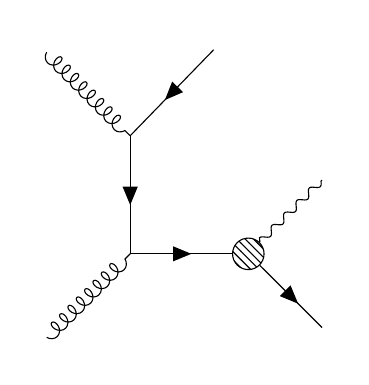
\begin{tikzpicture}
  \begin{feynman}
    \vertex[blob, minimum size=0.4cm] (v1) {};
    \vertex[left=of v1] (v6);
    \vertex[above=of v6] (v7);
    \vertex[above left=of v7] (p7) {\(\Pg\)};
    \vertex[above right=of v7] (v8) {\(\overline \Ptop\)};
    \vertex[below left=of v6] (p10) {\(\Pg\)};
    \vertex[above right=of v1] (p11) {\(\PZ\)};
    \vertex[below right=of v1] (p12) {\(\Ptop\)};

    \diagram* {
      (p7) -- [gluon] (v7) -- [fermion] (v6),
      (p10) -- [gluon] (v6) -- [fermion, edge label=\(\Ptop\)] (v1),
      (v8) -- [fermion] (v7),
      (p11) -- [boson] (v1) -- [fermion] (p12),
    };
  \end{feynman}
\end{tikzpicture}
}}
        \\
        \midrule
        \textbf{Tops + W (\ttW)}&
        \only<1>{\resizebox{2.5cm}{!}{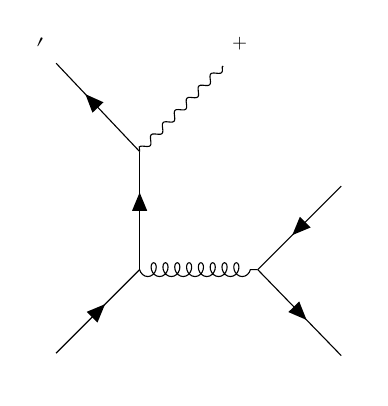
\begin{tikzpicture}
  \begin{feynman}
    \vertex (v1);

    \vertex[left=of v1] (v6);
    \vertex[above=of v6] (v7);
    \vertex[above left=of v7] (p7) {\(\overline \Pq^\prime\)};
    \vertex[above right=of v7] (v8) {\(\PW^+\)};
    \vertex[below left=of v6] (p10) {\(\Pq\)};
    \vertex[above right=of v1] (p11) {\(\Ptop\)};
    \vertex[below right=of v1] (p12) {\(\overline \Ptop\)};

    \diagram* {
      (p7) -- [anti fermion] (v7) -- [anti fermion] (v6),
      (p10) -- [fermion] (v6) -- [gluon, edge label=\(\Pg\)] (v1),
      (v8) -- [boson] (v7),
      (p11) -- [fermion] (v1) -- [fermion] (p12),
    };
  \end{feynman}
\end{tikzpicture}
}}
        \only<2>{\resizebox{!}{2.5cm}{\begin{tikzpicture}
  \begin{feynman}
    \diagram [horizontal=a to b] {
      i1 [particle=\(\Pq^\prime\)] -- [fermion] a -- [fermion] i2 [particle=\(\overline \Pq\)],
      a -- [boson, edge label'=\(\PW^-\)] b,
      c [blob, minimum size=0.4cm] -- [anti fermion, edge label=\(\Pb\)] b -- [anti fermion] f2 [particle=\(\overline \Ptop\)],
    };

    \vertex [above right=of c] (d) {\(\PW^-\)};
    \vertex [below right=of c] (e) {\(\Ptop\)};

    \diagram* {
      (d) -- [boson] (c) -- [fermion] (e);
    };
  \end{feynman}
\end{tikzpicture}
}}
      \end{tabular}
    \end{column}
  \end{columns}
  \centering
\end{frame}

\begin{frame}[standout]
  EFT is a useful tool for searching for NP

  \vspace{1cm}

  Some dimension-six operators would affect \ttW and \ttZ cross sections

  \vspace{1cm}

  Analysis goal: use \ttW and \ttZ cross section measurements to constrain their Wilson coefficient values
\end{frame}

\section{Experiment}

\begin{frame}{The Compact Muon Solenoid}
  \centering
  \includegraphics[width=11cm]{figures/cms_complete_labelled}
\end{frame}

\begin{frame}{The Compact Muon Solenoid}
  \centering
  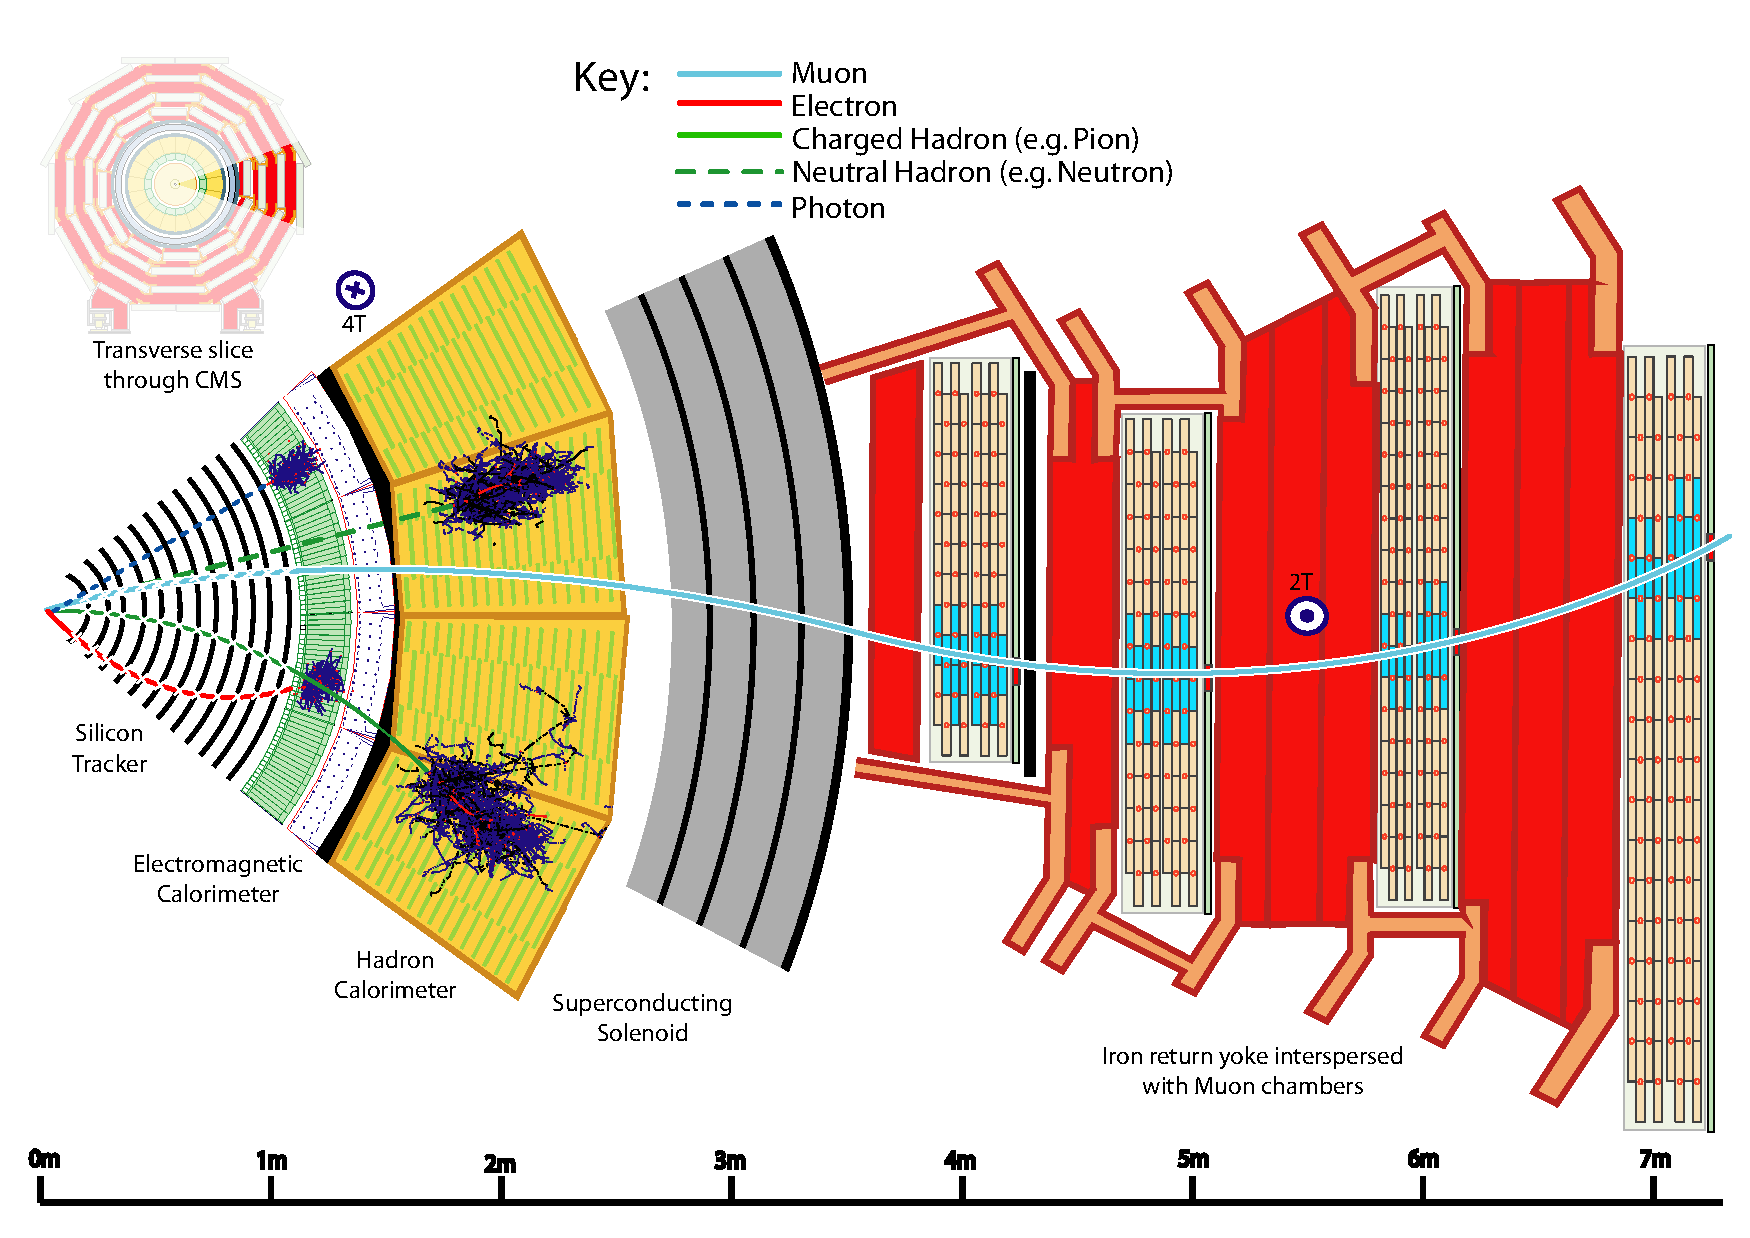
\includegraphics[width=11cm]{figures/cms_slice_white}
\end{frame}


\section{Cross section measurements}

\begin{frame}{What does \ttW and \ttZ look like?}
  \centering
  \resizebox{10cm}{!}{
    \feynmandiagram [horizontal=a to b] {
  a [particle=\(\Ptop\)] -- [fermion] b -- [fermion] d [particle=\(\Pb\)],
  b -- [boson] c [particle=\(\PW\)],
};
\feynmandiagram [horizontal=a to b] {
  a [particle=\(\PW\)] -- [boson] b -- [anti fermion] d [particle={\(\overline \nu, \ell^+, \overline \Pq\)}],
  b -- [fermion] c [particle={\(\ell^-, \nu, \Pq^\prime\)}],
};
\feynmandiagram [horizontal=a to b] {
  a [particle=\(\PZ\)] -- [boson] b -- [anti fermion] d [particle={\(\overline \nu, \ell^+, \overline \Pq\)}],
  b -- [fermion] c [particle={\(\nu, \ell^-, \Pq\)}],
};

  }

  We do not see the tops, Zs, and Ws directly: they decay before they reach the detector. So we look for the stuff they decay to.

  $\rightarrow$ Focus on \textbf{multilepton signatures:} at least one lepton ($\Plep = \mu, \Pe$) from the top and one from the W or Z. Fewer events, but cleaner signature!
\end{frame}

\begin{frame}{Analysis signatures and selection}
  \begin{columns}
    \begin{column}{.5\linewidth}
      \centering
      \resizebox{\linewidth}{!}{
        \input{figures/diagrams/3l-ttZ}
      }
      \Large
      3\Plep \ttZ

      $\ttZ \rightarrow (\Pb\ell\nu)(\Pb\Pj\Pj)(\ell\ell)$

    \end{column}
    \begin{column}{.5\linewidth}
      \centering
      \resizebox{\linewidth}{!}{
        \begin{tabular}{lC{3.5cm}}
          \toprule
          & 3\Plep \ttZ \\
          \midrule
          lepton \pT             & $>\num{10}/\num{20}/\SI{40}{GeV}$                               \\
          jets\tnote{a}          & $2, 3, > 3$                                                     \\
          b-tagged jets\tnote{a} & $0, 1, > 1$                                                     \\
          Z window               & OSSF pair with \mbox{$\abs{M_{\ell\ell} - M_Z} < \SI{10}{GeV}$} \\
          \bottomrule
        \end{tabular}
      }
    \end{column}
  \end{columns}
\end{frame}

\begin{frame}{Analysis signatures and selection}
  \begin{columns}
    \begin{column}{0.5\linewidth}
      \centering
      \resizebox{\linewidth}{!}{
        \tikzfeynmanset{
  small,
}
\begin{tikzpicture}
  \begin{feynman}
    \diagram [horizontal'=v1 to p4,tree layout,sibling distance=6mm,level distance=15mm] {
      v1 -- [fermion,edge label'=\(\Ptop\)] v3
         -- [fermion] p1 [particle=\(\Pb\)],
      v3 -- [boson,edge label=\(\PW^+\)] v5
         -- [fermion] p2 [particle=\(\nu\)],
      v5 -- [anti fermion] p3 [particle=\(\Plep^+\)],
      v1 -- [boson,edge label=\(\PZ\)] v4
         -- [fermion] p4 [particle=\(\Plep^-\)],
         v4 -- [anti fermion] p5 [particle={\(\Plep^+\)}],
    };

    \vertex[left=20mm of v1] (v6);
    \vertex[above=20mm of v6] (v7);
    \vertex[above left=4mm and 20mm of v7] (p7) {\(\Pg\)};
    \vertex[above right=4mm and 20mm of v7] (v8);
    \vertex[above right=4mm and 20mm of v8] (p8) {\(\overline \Pb\)};
    \vertex[below right=4mm and 20mm of v8] (p9);
    \vertex[below left=4mm and 20mm of v6] (p10) {\(\Pg\)};
    \vertex[below right=4mm and 20mm of p9] (p11) {\(\Plep^-\)};
    \vertex[above right=4mm and 20mm of p9] (p12) {\(\overline \nu\)};

    \diagram* {
      (p7) -- [gluon] (v7) -- [fermion] (v6),
      (p11) -- [anti fermion] (p9) -- [anti fermion] (p12),
      (p10) -- [gluon] (v6) -- [fermion, edge label=\(\Ptop\)] (v1),
      (p8) -- [fermion] (v8) -- [boson, edge label=\(\PW^-\)] (p9),
      (v8) -- [fermion, edge label=\(\overline \Ptop\)] (v7),
    };
  \end{feynman}
  \begin{pgfonlayer}{background}
      \node[fill=blue,fill opacity=0.4,circle,inner sep=1mm,fit=(p4)] {};
      \node[fill=blue,fill opacity=0.4,circle,inner sep=1mm,fit=(p5)] {};
      \node[fill=blue,fill opacity=0.4,circle,inner sep=1mm,fit=(p11)] {};
      \node[fill=blue,fill opacity=0.4,circle,inner sep=1mm,fit=(p3)] {};
  \end{pgfonlayer}
\end{tikzpicture}

      }
      \Large
      4\Plep \ttZ

      $\ttZ \rightarrow (\Pb\ell\nu)(\Pb\ell\nu)(\ell\ell)$
    \end{column}
    \begin{column}{0.5\linewidth}
      \resizebox{\linewidth}{!}{
        \begin{tabular}{lC{3.5cm}}
          \toprule
          & 4\Plep \ttZ \\
          \midrule
          lepton \pT                   &  $>\num{10}/\num{10}/\num{10}/\SI{40}{GeV}$ \\
          jets\tnote{a}                &  $\ge 2$ \\
          b-tagged jets\tnote{a}       &  $0, \ge 1$ \\
          Z window                     &  OSSF pair with \mbox{$\abs{M_{\ell\ell} - M_Z} < \SI{20}{GeV}$} and veto on additional OSSF pair \\
          \bottomrule
        \end{tabular}
      }
    \end{column}
  \end{columns}
\end{frame}

\begin{frame}{Analysis signatures and selection}
  \begin{columns}
    \begin{column}{.5\linewidth}
      \centering
      \resizebox{\linewidth}{!}{
        \input{figures/diagrams/ss-ttW}
      }
      \Large
      same-sign \ttW

      $\ttW \rightarrow (\Pb\ell\nu)(\Pb\Pj\Pj)(\ell\nu)$
    \end{column}
    \begin{column}{.5\linewidth}
      \centering
      \resizebox{\linewidth}{!}{
        \begin{tabular}{lc}
          \toprule
                                                                            & SS \ttW \\
          \midrule
        lepton \pT \(\left\{\begin{array}{l}\Pe\\\Pmu\\\end{array}\right.\) & \(\begin{array}{l}>\SI{27/40}{\GeV}\\>\SI{25}{\GeV}\\\end{array}\) \\
          jets\tnote{a}                                                     & $2, 3, > 3$ \\
          b-tagged jets\tnote{a}                                            & $1, > 1$ \\
          Z window                                                          & $\abs{M_{ee} - M_Z} > \SI{15}{GeV}$ \\
          \pTmiss                                                           & $> \SI{30}{GeV}$ \\
          % BDT\tnote{a}                                                      & $D > 0$, $D < 0$ \\
          % charge\tnote{a}                                                   & $\ell^+\ell^+, \ell^-\ell^-$ \\
          \bottomrule
        \end{tabular}
    }
    \end{column}
  \end{columns}
\end{frame}

\begin{frame}{Backgrounds}
  %TODO Add feynman diagrams
  Nonprompt leptons (SS \ttW, 3\Plep \ttZ)
  \begin{itemize}
    \item Leptons from b decays, misidentified jets, photon conversions, etc (mostly from \ttbar + jets)
    \item Estimated from data
      \begin{itemize}
        \item Measure rate $f_\text{TL}$ loose leptons pass tight criteria in \textbf{measurement region} enriched with nonprompt leptons
        \item Weight \textbf{application region} events which pass full selection, except that at least one lepton passes loose selection but fails tight selection by $f_\text{TL}$
      \end{itemize}
  \end{itemize}
  Charge misidentification (SS \ttW)
  \begin{itemize}
    \item Charge of one electron is misidentified
    \item Misidentification rate measured in simulation and validated in data $\PZ \rightarrow \Pe\Pe$ events
  \end{itemize}
\end{frame}

\begin{frame}{Backgrounds}
  %TODO add feynman diagrams
  %TODO explain irreducible
  WZ (SS \ttW, 3\Plep \ttZ) and ZZ (4\Plep \ttZ)
  \begin{itemize}
    \item Estimated from simulation
    \item Measure data/MC correction factor in WZ enriched control region
    \item ZZ validated in enriched control region
  \end{itemize}
  Rare and \ttX (SS \ttW, 3\Plep \ttZ, 4\Plep \ttZ)
  \begin{itemize}
    \item Generally small contribution
    \item Estimated from simulation
  \end{itemize}
\end{frame}

\begin{frame}{Signal extraction}
      \centering
      \begin{tabular}{C{4cm}|C{7cm}}
      \includegraphics[height=3.5cm]{figures/thirteen-TeV/bdt} & \includegraphics[height=3.5cm]{figures/thirteen-TeV/3l-ttZ-mll} \includegraphics[height=3.5cm]{figures/thirteen-TeV/postfit-4l} \\
      \textbf{SS \ttW} & \textbf{3\Plep \ttZ, 4\Plep \ttZ} \\
      Categorize by charge to take advantage of W charge asymmetry; use BDT to enhance sensitivity &
        Cut on Z mass window and b jets \\
    \end{tabular}
\end{frame}

\begin{frame}{Characterizing the data}
  \centering
  signal strength $\mu=\frac{\sigma}{\sigma_\text{SM}}$
  \includegraphics[height=6.5cm]{figures/cartoon-1}
\end{frame}

\begin{frame}{Characterizing the data}
  \addtocounter{framenumber}{-1}
  \centering
  signal strength $\mu=\frac{\sigma}{\sigma_\text{SM}}$
  \includegraphics[height=6.5cm]{figures/cartoon-2}
\end{frame}

\begin{frame}{Characterizing the data}
  \addtocounter{framenumber}{-1}
  \centering
  signal strength $\mu=\frac{\sigma}{\sigma_\text{SM}}$
  \includegraphics[height=6.5cm]{figures/cartoon-3}
\end{frame}

\begin{frame}{Results}
  \centering
\includegraphics[width=4.5cm]{figures/thirteen-TeV/sm-2d-only}
\begin{align*}
  \sigma(\text{pp} \rightarrow \ttZ) &= 0.99^{+0.09}_{-0.08}\text{(stat)}^{+0.12}_{-0.10}\text{(syst)}\,\text{pb} \\
  \sigma(\text{pp} \rightarrow \ttW) &= 0.77^{+0.12}_{-0.11}\text{(stat)}^{+0.13}_{-0.12}\text{(syst)}\,\text{pb} \\
  \sigma(\text{pp} \rightarrow \ttW^{+}) &= 0.58\pm{0.09}\text{ (stat) }^{+0.09}_{-0.08}\text{ (syst) }\,\text{pb} \\
  \sigma(\text{pp} \rightarrow \ttW^{-}) &= 0.19\pm{0.07}\text{ (stat) }\pm{0.06}\text{ (syst) }\,\text{pb}
\end{align*}
\end{frame}

\section{Effective field theory interpretation}

\begin{frame}{Why is this hard?}
  \begin{enumerate}
    \item There are 59 dimension six operators--- multiple couplings may be enhanced, and operators may interfere with each other
    \item EFT might affect \ttW and \ttZ kinematics
  \end{enumerate}

  In this work\footnote{\emph{Most} of this work--- later I will show preliminary steps toward relaxing assumption 1) and ideas for tackling 2)}, we make two simplifications:
  \begin{enumerate}
    \item Study couplings independently
    \item Assume EFT only affects cross sections (negligible effect on kinematics)
  \end{enumerate}
\end{frame}

\begin{frame}{General strategy}
  % TODO fix math font
  How to calculate scaling of $\sigma_{\ttW}$ and $\sigma_{\ttZ}$ as a function of the Wilson coefficients?
  \centering
  \begin{overlayarea}{\textwidth}{6cm}
    \only<1>{
      \begin{equation*}
        \mathcal{M}_\text{NP+SM} = \mathcal{M}_\text{SM} + \sum c_i\mathcal{M}_i
      \end{equation*}
    }
    \only<2>{
      \begin{equation*}
        \xcancel{\mathcal{M}_\text{NP+SM} = \mathcal{M}_\text{SM} + \sum c_i\mathcal{M}_i}
      \end{equation*}
      \begin{equation*}
        \mathcal{M}_\text{SM+NP} = \mathcal{M}_\text{SM} + c_1\mathcal{M}_1
      \end{equation*}
      \begin{align*}
        \mu(c_1)= \frac{\sigma_\text{SM+NP}(c_1)}{\sigma_\text{SM}} = \frac{\sigma_\text{SM+NP}(c_1)}{\sigma_\text{SM+NP}(0)} =
        &\propto \frac{\abs{\mathcal{M}_\text{SM+NP}}^2}{\abs{\mathcal{M}_\text{SM}}^2}\\
        &\propto \frac{\abs{\mathcal{M}_\text{SM} + c_1\mathcal{M}_1}^2}{\abs{\mathcal{M}_\text{SM}}^2}\\
        &\propto s_0 + s_1c_1 + s_2c_1^2
      \end{align*}
    }
  \end{overlayarea}
\end{frame}

\begin{frame}{General strategy}
  \centering
  What does $\mu(c_1)$ look like?

  \includegraphics[width=0.6\textwidth]{figures/scaling/cuG}
\end{frame}

\begin{frame}{General strategy}
  \centering
  % $\mu(c_1)= \frac{\sigma_\text{SM+NP}(c_1)}{\sigma_\text{SM}} = \frac{\sigma_\text{SM+NP}(c_1)}{\sigma_\text{SM+NP}(0)}$
  \includegraphics[height=5.5cm]{figures/cartoon-3}

  Find best-fit $c_1$ (constrained by $\mu(c_1) = s_0 + s_1c_1 + s_2c_1^2$)
\end{frame}

\begin{frame}{Eight TeV analysis\footnote{\tiny V. Khachatryan et al. ``Observation of top quark pairs produced in association with a vector boson in pp collisions at $\sqrt{s}$ = 8 TeV''. In: JHEP 01 (2016), p. 096. doi:10.1007/JHEP01(2016)096.}}
  Select five operators because they have a small effect on inclusive Higgs boson and \ttbar, and a large effect on \ttZ, \ttW, or both
  \vspace{1cm}

  \resizebox{\linewidth}{!}{
    \begin{tabular}{lccc}
      \toprule
      Coefficient & Best fit point(s)  & \SI{68}{\percent} CL                 & \SI{95}{\percent} CL \\
      \midrule
      \cuB        & $-0.07$ and $0.07$ & $[-0.11, 0.11]$                      & $[-0.14, 0.14]$\\
      \cthreeW    & $-0.28$ and $0.28$ & $[-0.36, -0.18]$ and $[0.18, 0.36]$  & $[-0.43, 0.43]$\\
      \cHu        & $-0.47$ and $0.13$ & $[-0.60, -0.23]$ and $[-0.11, 0.26]$ & $[-0.71, 0.37]$\\
      \cHQ        & $-0.09$ and $0.41$ & $[-0.22, 0.08]$ and $[0.24, 0.54]$   & $[-0.31, 0.63]$\\
      \cpHQ       & $0.12$             & $[-0.07, 0.18]$                      & $[-0.33, -0.24]$ and $[-0.02, 0.23]$\\
      \bottomrule
    \end{tabular}
  }
\end{frame}

\begin{frame}{Thirteen TeV analysis: improvements}
  \begin{itemize}
    \item Removed NP couplings to light quarks\footnote{Big thanks to Adam Martin for providing the new Feynrules implementation and much additional help} because they are highly constrained by other measurements
    \item Added scaling for \ttH
    \item Improved range-finding for parameterization
    \item More sophisticated selection of operators we care about
\end{itemize}
\end{frame}


\begin{frame}{\resizebox{\linewidth}{!}{Eliminate operators with large effect on precisely measured processes}}
  Define extreme signal scaling  $\mu_\text{e}(c_1)$ to be $\mu(c_1)$ evaluated at the $c_1$ which maximizes $\abs{\mu(c_1) - 1}$ within the range of $c_1$ corresponding to $2\sigma$ sensitivity

  Exclude operators producing $\abs{\mu_\text{e} - 1} > 0.7$ for any of $\ttbar$, inclusive Higgs, DY, WW, and WZ

  \centering
  \resizebox{0.75\linewidth}{!}{
   \begin{tabular}{lrrrrrrr}
     \toprule
                          &  $\mu_\text{e,\ttbar}$ & $\mu_\text{e,H}$ & $\mu_\text{e,DY}$ & $\mu_\text{e,ZZ}$ & $\mu_\text{e,WZ}$ & $\mu_\text{e,WW}$ \\
     \midrule
     $\widetilde{c}_{HB}$ &  $1.0$                 & $1.0$            & $1.0$             & $1.1$             & $5.0$             & $4.6$ \\
     $\bar{c}_{G}$        &  $0.6$                 & $1610.7$         & $1.1$             & $5.2$             & $1.0$             & $2.5$ \\
     $\widetilde{c}_{G}$  &  $1.0$                 & $739.4$          & $1.0$             & $2.9$             & $1.0$             & $1.7$ \\
     $\bar{c}_{Hd}$       &  $1.0$                 & $1.0$            & $1.3$             & $1.1$             & $1.0$             & $2.8$ \\
     $\bar{c}_{HW}$       &  $1.0$                 & $1.0$            & $1.0$             & $1.0$             & $1.7$             & $1.1$ \\
     $\widetilde{c}_{3W}$ &  $1.0$                 & $1.0$            & $1.0$             & $1.0$             & $7.9$             & $2.6$ \\
     $\bar{c}_{3W}$       &  $1.0$                 & $1.0$            & $1.0$             & $1.0$             & $7.9$             & $2.6$ \\
     $\bar{c}_{WW}$       &  $1.0$                 & $1.0$            & $1.0$             & $1.0$             & $2.0$             & $1.2$ \\
     \bottomrule
   \end{tabular}
 }
\end{frame}

\begin{frame}{Eliminate operators with large effect on background yields}
  Checked 13 processes, worst offenders: triboson, VH, \ttX. Eliminate them for now, but promising direction for future work!

  \resizebox{\linewidth}{!}{
    \begin{threeparttable}
      \begin{tabular}{lrrrrrrrrr}
        \toprule
        &  \multicolumn{5}{c}{$\text{T}_\text{SM}=218$} & \multicolumn{4}{c}{$\text{T}_\text{SM}=175$} \\
        \cmidrule(lr){2-6} \cmidrule(lr){7-10}
                  & $\Delta_\text{WWW}$ & $\Delta_\text{WZZ}$ & $\Delta_\text{ZZZ}$ & $\Delta_\text{WWZ}$ & $\Delta_\text{VH}$ & $\Delta_\text{tZq}$ & $\Delta_\text{tHq}$ & $\Delta_\text{tHW}$  & $\Delta_\text{tWZ}$ \\
        \midrule
        \cHB  & $60$   & $7$   & $273$ & $1080$ & $3355$  & $48$   & $0$    & $0$   & $0$ \\
        \tcHW & $2053$ & $950$ & $417$ & $1017$ & $36709$ & $37$   & $805$  & $47$  & $0$ \\
        \cHud & $0$    & $0$   & $0$   & $43$   & $0$     & $1818$ & $1677$ & $340$ & $20$ \\
        \cHQ  & $0$    & $0$   & $41$  & $225$  & $1281$  & $258$  & $0$    & $0$   & $4$ \\
        \cB   & $0$    & $1$   & $304$ & $1750$ & $4178$  & $0$    & $0$    & $0$   & $0$ \\
        \tcA  & $0$    & $9$   & $835$ & $1959$ & $20518$ & $0$    & $0$    & $0$   & $0$ \\
        \cpHQ & $0$    & $0$   & $24$  & $81$   & $772$   & $1688$ & $1504$ & $269$ & $16$ \\
        \cu   & $0$    & $0$   & $0$   & $0$    & $0$     & $0$    & $292$  & $45$  & $0$ \\
        \bottomrule
      \end{tabular}
      \begin{tablenotes}
      \item[1] Yields differences are calculated as $\Delta = \sum_i \text{N}^i_\text{SM}(\mu_\text{e} - 1)$, where $\text{N}^i_\text{SM}$ refers to the expected SM yield in a particular channel, and the sum is over $i$ channels.
        % \item[2] Only scaling effects due to operators which pass the requirement that $\abs{\mu_\text{e} - 1} < 0.7$ for \ttbar, inclusive Higgs, WW, and WZ, but have an unacceptably large effect on background yields are tabulated.
      \item[3] $\text{T}_\text{SM}$ is the sum of expected SM yields over channels and the given process group: $\text{T}_\text{SM} = \sum_{i,p} \text{N}^{i,p}_\text{SM}$.
      \end{tablenotes}
    \end{threeparttable}
  }
\end{frame}

\begin{frame}{Results}
  \centering
  \begin{overlayarea}{\textwidth}{7cm}
  \resizebox{!}{0.42\textheight}{
    \includegraphics[height=\textheight]{figures/thirteen-TeV/NP/mu/cuW}\hspace{5mm}
    \includegraphics[height=\textheight]{figures/thirteen-TeV/NP/nll/cuW}\hspace{5mm}
    \includegraphics[height=\textheight]{figures/thirteen-TeV/NP/2D/ttZ_ttW_2D_1D_cuW}
  }
  \only<1>{
    \centering
  Eight survivors: \cH, \tcthreeG, \cthreeG, \cuG, \cuB, \cHu, and \ctwoG \\
}
  \only<2>{
    \resizebox{!}{0.42\textheight}{
      \includegraphics[height=\textheight]{figures/thirteen-TeV/NP/mu/c3G}\hspace{5mm}
      \includegraphics[height=\textheight]{figures/thirteen-TeV/NP/nll/c3G}\hspace{5mm}
      \includegraphics[height=\textheight]{figures/thirteen-TeV/NP/2D/ttZ_ttW_2D_1D_c3G}
    }
  }
  \only<3>{
    \centering
    \vspace{5mm}
    \resizebox{0.9\linewidth}{!}{
      \begin{tabular}{lrrr}
        \toprule
        Wilson coefficient                              & Best fit $[\si{TeV}^{-2}]$ & \SI{68}{\percent} CL $[\si{TeV}^{-2}]$ & \SI{95}{\percent} CL $[\si{TeV}^{-2}]$\\
        \midrule
        $\cuW/\Lambda^2$                                & $1.7$                                                 & $[-2.4, -0.5] \cup [0.4, 2.4]$                       & $[-2.9, 2.9]$ \\
        $\abs{\cH/\Lambda^2 - 16.8\ \mathrm{TeV}^{-2}}$ & $15.6$                                                & $[0, 23.0]$                                          & $[0, 28.5]$ \\
        $\abs{\tcthreeG/\Lambda^2}$                     & $0.5$                                                 & $[0, 0.7]$                                           & $[0, 0.9]$ \\
        $\cthreeG/\Lambda^2$                            & $-0.4$                                                & $[-0.6, 0.1] \cup [0.4, 0.7]$                        & $[-0.7, 1.0]$ \\
        $\cuG/\Lambda^2$                                & $0.2$                                                 & $[0, 0.3]$                                           & $[-1.0, -0.9] \cup [-0.3, 0.4]$ \\
        $\abs{\cuB/\Lambda^2}$                          & $1.6$                                                 & $[0, 2.2]$                                           & $[0, 2.7]$ \\
        $\cHu/\Lambda^2$                                & $-9.3$                                                & $[-10.3, -8.0] \cup [0, 2.1]$                        & $[-11.1, -6.5] \cup [-1.6, 3.0]$ \\
        $\ctwoG/\Lambda^2$                              & $0.4$                                                 & $[-0.9, -0.3] \cup [-0.1, 0.6]$                      & $[-1.1, 0.8]$ \\
        \bottomrule
      \end{tabular}
    }
  }
\end{overlayarea}
\end{frame}

\begin{frame}{$\mu(c_i)$ parameterization with multiple parameters}
  Considering the effects of operators simultaneously is more physically meaningful. Example for three:
  \footnotesize
  {\setlength{\mathindent}{-5mm}
    \begin{equation*}
      \mu(c_1, c_2, c_3) = \frac{\sigma_\text{SM+NP}(c_1, c_2, c_3)}{\sigma_\text{SM}}
    \end{equation*}
  \vspace{-5mm}
  \begin{align*}
  \quad &\propto \frac{\lvert\mathcal{M}_\text{SM} + c_1\mathcal{M}_1 + c_2\mathcal{M}_2 + c_3\mathcal{M}_3\rvert^2}{\lvert\mathcal{M}_\text{SM}\rvert^2} \\
    &\propto \underbrace{s_0}_{\text{const.}} + \underbrace{s_1 c_1 + s_2 c_2 +s_3 c_3}_{\text{linear}} + \underbrace{s_4 c_1^2 + s_5 c_2^2 + s_6 c_3^2}_{\text{quadratic}} + \underbrace{s_7 c_1 c_2 + s_8 c_1 c_3 + s_9 c_2 c_3}_{\text{mixed}}
  \end{align*}
  }
  If there are $d$ operators, there will be $N_s$ structure constants, where
  \begin{equation*}
    N_s = 1 + 2d + \frac{d}{2}(d - 1)
  \end{equation*}
\end{frame}

\begin{frame}{$\mu(c_i)$ parameterization in two dimensions}
  \begin{overlayarea}{\textwidth}{7cm}
    \includegraphics[width=\textwidth]{figures/thirteen-TeV/NP/c2G_cH} \\
    \only<2>{\includegraphics[width=\textwidth]{figures/thirteen-TeV/NP/c2G_cH_mg}}
  \end{overlayarea}
\end{frame}

\begin{frame}{Thirteen TeV analysis: simultaneous fit (preliminary!)}
  \begin{columns}
    \begin{column}{.5\linewidth}
      \centering
      \includegraphics[width=\linewidth]{figures/thirteen-TeV/nll/c2G_cuW}
    \end{column}
    \begin{column}{.5\linewidth}
      \centering
      CL surface `bounding box' for 8D simultaneous fit

      \resizebox{\linewidth}{!}{
        \begin{tabular}{lccc}
          \toprule
          & \SI{0.68}{\percent} CL / $\si{TeV}^{-2}$ & \SI{0.95}{\percent} CL / $\si{TeV}^{-2}$ \\
          \midrule
          $\bar{c}_{2G}$$/\Lambda^2$       & [-10.4, 10.0]       & [-12, 12] \\
          $\bar{c}_{3G}$$/\Lambda^2$       & [-9.2, 8.6]         & [-10.4, 9.9] \\
          $\bar{c}_{H}$$/\Lambda^2$        & [-25, 52]           & [-31, 57] \\
          $\bar{c}_{Hu}$$/\Lambda^2$       & [-13, 6.2]          & [-14, 7.3] \\
          $\bar{c}_{uB}$$/\Lambda^2$       & [-7.8, 7.3]         & [-8.5, 7.9] \\
          $\bar{c}_{uG}$$/\Lambda^2$       & [-1.4, 1.0]         & [-1.6, 1.1] \\
          $\bar{c}_{uW}$$/\Lambda^2$       & [-7.5, 6.8]         & [-8.2, 7.4] \\
          $\widetilde{c}_{3G}$$/\Lambda^2$ & [-1.3, 1.3]         & [-1.4, 1.4] \\
          \bottomrule
        \end{tabular}
      }
    \end{column}
  \end{columns}
\end{frame}

\section{Future directions}

\begin{frame}{Parameterized matrix element reweighting}
  Matrix element reweighting: `recycle' simulated events to model different hypothesis by weighting events:
  \begin{equation*}
    w_\text{new} = w_\text{orig} \frac{\abs{\mathcal{M}_\text{new}}^2}{\abs{\mathcal{M}_\text{orig}}^2}
  \end{equation*}
  Bad news: `combinatoric explosion' still a problem! Assuming 32 bits of memory per weight: weights for one event evaluated at just 10 values per parameter in a 15 dimensional parameter space would require $10^{15}$ x $\SI{32}{bits} = \SI{4000}{TB}$!
\end{frame}

\begin{frame}{Parameterized matrix element reweighting}
  \begin{equation*}
    w_\text{new}(c_1) = w_\text{orig} \frac{\abs{\mathcal{M}_\text{SM} + c_1\mathcal{M}}^2}{\abs{\mathcal{M}_\text{orig}}^2} = w_\text{orig} \frac{s_0 + s_1c_1 + s_2c_1^2}{\abs{\mathcal{M}_\text{orig}}^2}
  \end{equation*}
  \begin{itemize}
    \item Before: parameterized $\mu(c_i)$ per-process\\Now: parameterize $w(c_i)$ per-event
    \item Need more, but they are cheap: \num{50000} parameterizations in 8D (one for each event) to 200 points: $\approx \SI{100}{seconds}$
    \item Preliminary look shows parameterization is able to well-reproduce `traditional' weights!
    \item Future work: how to choose reference model, handle uncertainties, etc... If these can be addressed, could perform `traditional' analysis, then apply reweighting to final discriminant histograms
  \end{itemize}
\end{frame}

\section{Conclusions}

\begin{frame}{Conclusion}
  \footnotesize
  \begin{itemize}
    \item Used \ttW and \ttZ cross section measurements to constrain Wilson coefficients of dimension-six operators (results consistent with SM)
    \item Challenging because of large phase space; (mostly) studied operators independently, and assumed only rates are affected
    \item Different combos of Wilson coefficient values can correspond to identical cross section scaling; this degeneracy is a challenge
    \item Identified large NP effects on triboson, \ttX, and VH processes-- hints at interesting direction for future work (fitting effects on more signal regions simultaneously helps break degeneracies)
    \item Building on experience parameterizing NP effects for one coefficient:
      \begin{itemize}
  \footnotesize
        \item Preliminary results in from simultaneous parameterization of multiple coefficients were presented
        \item It was shown how the approach can be extended to `recycle' simulation without large storage requirements; this could be used in detector-level analyses, benefit from kinematic handles to further break degeneracies
      \end{itemize}
  \end{itemize}
    % \item  For a given process, many combinations of Wilson coe cient values may corre- spond to identical scaling of the cross section. These surfaces of equal scaling are a fundamental degeneracy that cannot be resolved using the approach taken in this dissertation.
  % f those problems can be addressed satisfactorily, then the pa- rameterization of the weights for each event can be determined and saved when an event is simulated. Detector-level analyses can proceed in the usual way, without restrictions regarding the use of advanced techniques such as MVAs. As a  nal step, the discriminant histograms can be reweighted to re ect a desired point in high-dimensional parameter space. This operation will be cheap enough that it could be performed for each step of the likelihood minimization.
\end{frame}

\appendix

\begin{frame}{The end: THANK YOU!}
  \begin{center}
    \footnotesize
    Stack overflow community

    Kevin Lannon, committee members, ND HEP group, Jason Slaunwhite, Andrew Brinkerhoff, Matthias Wolf, Kenyi Paolo Hurtado Anampa, all the students who have helped me

    13 TeV ttV team: Didar Dobur, Illia Khvastunov, Mirena Paneva, and Deniz Poyraz

    Douglas Thain and his Cooperative Computing Lab team

    Serguei Federov, Paul Brenner, Scott Hampton, and the CRC team

    Theorists who put up with many questions: Adam Martin, Fatimah Elahi, Landon Lehman, Ayan Paul, Joe Bramante, Brian Ostdiek, Fabio Maltoni, Eleni Vryonidou

    LHC accelerator team, CMS Collaboration

    Shari Herman
  \end{center}
\end{frame}

% \begin{frame}[standout]
%   backup
% \end{frame}

%\begin{frame}{Tweaks}
%  \footnotesize
%    I would like to request approval for a few tweaks to my dissertation:
%    \begin{itemize}
%      \item Yield difference tables 7.6 and 7.7:
%        \begin{itemize}
%          \item Corrected columns for VH and tG, which were accidentally set to 0
%          \item Added SM yields for more meaningful comparison
%        \end{itemize}
%      \item Added conclusions (similar to talk's conclusion slide)
%      \item Added acknowledgments
%      \item Add short (1 page) appendix on analysis reproducibility + references to computing work
%      \item Added uncertainties to the structure constant tables
%      \item Clarified Fig 7.13 and its description
%      \item Appendix A:
%        \begin{itemize}
%          \item For the 2D NLL scans, added plots profiling the remaining coefficients instead of fixing them to 0
%          \item Added 2D scaling scans at the best-fit point
%        \end{itemize}
%    \end{itemize}
%\end{frame}

%\begin{frame}
%  This control sample consists
%of events with a single lepton and at least one jet, where the lepton and jets are separated by
%∆R > 1. We suppress the prompt lepton contamination, mostly from W+jets, by requiring
%pmiss < 20 GeV and MT < 20 GeV, where MT is the transverse mass constructed using pmiss TT
%and the selected lepton.
%\end{frame}

%\begin{frame}{Parameterized matrix element reweighting}
%  \centering
%  Preliminary parameterizations look promising!
%  \includegraphics[width=0.7\textwidth]{figures/reweighting/weight_vs_err_8d}

%  Future work: how to choose reference model, properly handle uncertainties, etc... If these problems can be addressed satisfactorily, could perform `traditional' analysis, then apply reweighting to final discriminant histograms
%\end{frame}

%\begin{frame}{Summary of selection}
%  \centering
%  \begin{tabularx}{\textwidth}{L{5cm}X}
%    \toprule
%    Requirement & Eliminated \\
%    \midrule
%    % \text{simulation problem} \quad\rightarrow\quad& \bar{c}_{2W},\,\bar{c}_{T},\, \bar{c}_{A}\\
%    No effect on \ttH, \ttZ, \ttW     & $\bar{c}_\text{l}$, $\bar{c}_\text{lB}$, $\bar{c}_\text{d}$, $\bar{c}_\text{2B}$, $\bar{c}_\text{lW}$, $\bar{c}_\text{dB}$, $\bar{c}_\text{dW}$, $\bar{c}'_\text{HL}$, $\bar{c}_\text{He}$, $\bar{c}_\text{dG}$, $\bar{c}_\text{6}$, $\bar{c}_\text{HL}$ \\
%    $\abs{\mu_{WZ} - 1} > 0.7$            & $\widetilde{c}_\text{HB}$, $\bar{c}_\text{T}$,\, $\widetilde{c}_\text{3W}$,\, $\bar{c}_\text{3W}$,\, $\bar{c}_\text{WW}$,\, $\bar{c}_\text{HW}$ \\
%    $\abs{\mu_{ZZ} - 1} > 0.7$            & $\bar{c}_\text{G}$, $\widetilde{c}_\text{G}$, $\bar{c}_\text{T}$ \\
%    $\abs{\mu_{WW} - 1} > 0.7$            & $\widetilde{c}_\text{HB}$, $\bar{c}_\text{G}$, $\widetilde{c}_\text{G}$, $\bar{c}_\text{T}$, $\bar{c}_\text{Hd}$, $\widetilde{c}_\text{3W}$, $\bar{c}_\text{3W}$ \\
%    $\abs{\mu_{tt} - 1} > 0.7$            & $\bar{c}_\text{uG}$, $\bar{c}_\text{G}$ \\
%    $\abs{\mu_{H} - 1} > 0.7$             & $\bar{c}_\text{G}$, $\widetilde{c}_\text{G}$ \\
%    Large effect on backgrounds & \cHB, \tcHW, \cHud, \cHQ, \cB, \tcA, \cpHQ, \cu \\
%    \bottomrule
%  \end{tabularx}

%  \vspace{5mm}
%  Eight survivors: \cH, \tcthreeG, \cthreeG, \cuG, \cuB, \cHu, and \ctwoG
%\end{frame}

%\begin{frame}{$\mu(c_i)$ parameterization in multiple dimensions}
%  Considering the effects of operators simultaneously is more physically meaningful. For two:
%  \begin{align*}
%    \sigma(c_1, c_2) &\propto \lvert\mathcal{M}_0 + c_1\mathcal{M}_1 + c_2\mathcal{M}_2\rvert^2 \\
%                     &\propto
%    \underbrace{s_0}_{\text{constant}} +
%    \underbrace{s_1 c_1 + s_2 c_2}_{\text{linear}} +
%    \underbrace{s_3 c_1^2 + s_4 c_2^2}_{\text{quadratic}} +
%    \underbrace{s_5 c_1 c_2}_{\text{mixed}}.
%    \label{eq:2d}
%  \end{align*}
%  And for three:
%  \begin{align*}
%    \sigma(c_1, c_2, c_3) &\propto \lvert\mathcal{M}_0 + c_1\mathcal{M}_1 + c_2\mathcal{M}_2 + c_3\mathcal{M}_3\rvert^2 \\
%                          &\propto \underbrace{s_0}_{\text{constant}} + \underbrace{s_1 c_1 + s_2 c_2 +s_3 c_3}_{\text{linear}} \\
%                          &+ \underbrace{s_4 c_1^2 + s_5 c_2^2 + s_6 c_3^2}_{\text{quadratic}} + \underbrace{s_7 c_1 c_2 + s_8 c_1 c_3 + s_9 c_2 c_3}_{\text{mixed}}
%  \end{align*}
%\end{frame}

%\begin{frame}{Effective Field Theory}
%  \centering
%  \resizebox{5cm}{!}{
%  \feynmandiagram [horizontal=a to b] {
%    i1 -- [fermion] a -- [fermion] i2,
%    a -- [boson] b,
%    f1 -- [fermion] b -- [fermion] f2,
%  };
%  \hspace{2cm}
%  \feynmandiagram [horizontal=i1 to f2] {
%    {i1, i2} -- [fermion] c [dot] -- [fermion] {f1, f2},
%  };
%}

%  \footnotesize
%  \begin{itemize}
%  \item Uncertainty principle: the larger the mass of a mediating particle, the shorter the range of the force
%  \item In EFT, take mass to be so large that the propagator connecting vertices is reduced to a point: simplified vertex is effective operator
%  \item Bonus: reduces $\approx \infty$ class of possible theories down to small set of EFT operators
%  \item At energies $E << \Lambda$ an operator's contribution will scale inversely with dimension\footnote{Dimensionality refers to the mass dimension. In natural units: $[m] = [E] = [p] = [x^{-1}] = [t^{-1}]$. The Lagrangian has dimension four, so $[\phi]=[A_\mu]=1$ and $[\psi]=3/2$.}
%, as higher-dimensional operators are suppressed by powers of $\Lambda$
%  \end{itemize}
%\end{frame}

%\begin{frame}{Thirteen TeV analysis}
%  %, no physics requirement to do it
%  We received feedback on 8 TeV paper:
%  \begin{itemize}
%    \item D6 operators were flavor-independent (equal coupling to all flavors) in 8 TeV analysis: this is a simplifying assumption
%    \item Z coupling to light quarks is highly constrained by other measurements $\rightarrow$ we removed 1st and 2nd gen quark couplings in the MadGraph implementation\footnote{Big thanks to Adam Martin For providing the new Feynrules implementation and a great deal of additional help}
%    \item Makes it harder to set limits because we are only sensitive to 3rd-gen couplings, but those are exactly what we want to probe
%\end{itemize}
%\end{frame}

%\begin{frame}{Operators with large effect on background yields}
%  Worst offenders: triboson, VH, \ttX. Eliminate them for now, but promising direction for future work!

%  \resizebox{\linewidth}{!}{
%    \begin{threeparttable}
%      \begin{tabular}{lrrrrrrrrrrrrrrrrr}
%        \toprule
%        & \multicolumn{3}{c}{$\text{T}\tnote{3}_\text{SM}=443$} & \multicolumn{5}{c}{$\text{T}_\text{SM}=218$} & \multicolumn{6}{c}{$\text{T}_\text{SM}=175$} & \multicolumn{2}{c}{$\text{T}_\text{SM}=1176$}\\
%        \cmidrule(lr){2-4} \cmidrule(lr){5-9} \cmidrule(lr){10-15} \cmidrule(lr){16-17}
%        & $\Delta_{\ttZ}$ & $\Delta_{\ttW}$ & $\Delta_{\ttH}$ & $\Delta_\text{WWW}$ & $\Delta_\text{WZZ}$ & $\Delta_\text{ZZZ}$ & $\Delta_\text{WWZ}$ & $\Delta_\text{VH}$ & $\Delta_\text{tZq}$ & $\Delta_\text{tHq}$ & $\Delta_\text{tHW}$ & $\Delta_{{\ttbar}{\ttbar}}$ & $\Delta_\text{tWZ}$ & $\Delta_\text{tG}$ & $\Delta_\text{WZ}$ & $\Delta_{ZZ}$     \\
%        \midrule
%        \cHB     & $135.2$         & $0.3$           & $36.5$          & $59.5$              & $8.6$               & $272.8$             & $1079.5$            & $3355.3$           & $47.8$              & $0.0$               & $0.0$               & $1.0$                       & $0.3$               & $0.0$              & $113.3$            & $1.3$   \\
%        \tcHW    & $75.1$          & $103.5$         & $2.1$           & $2052.7$            & $950.4$             & $416.7$             & $1017.2$            & $36709.2$          & $37.0$              & $804.6$             & $47.3$              & $0.0$                       & $0.4$               & $0.0$              & $260.2$            & $8.6$   \\
%        \cHud    & $135.5$         & $0.0$           & $35.6$          & $0.0$               & $0.0$               & $0.0$               & $42.7$              & $0.0$              & $1818.3$            & $1676.5$            & $339.6$             & $0.5$                       & $19.5$              & $0.0$              & $0.0$              & $0.0$   \\
%        \cHQ     & $-175.1$        & $2.7$           & $3.3$           & $0.0$               & $0.0$               & $41.2$              & $224.7$             & $1280.5$           & $257.7$             & $0.0$               & $0.0$               & $3.4$                       & $4.2$               & $0.0$              & $0.0$              & $90.1$ \\
%        \cB      & $135.8$         & $0.0$           & $35.1$          & $0.0$               & $0.6$               & $304.2$             & $1750.1$            & $4177.8$           & $0.0$               & $0.0$               & $0.0$               & $1.0$                       & $0.0$               & $0.0$              & $0.0$              & $0.8$   \\
%        \tcA     & $145.9$         & $0.0$           & $8.2$           & $0.0$               & $8.8$               & $835.2$             & $1958.5$            & $20517.7$          & $0.0$               & $0.0$               & $0.0$               & $0.1$                       & $0.0$               & $0.0$              & $0.0$              & $9.3$   \\
%        \cpHQ    & $-149.6$        & $2.5$           & $47.5$          & $0.0$               & $0.0$               & $24.4$              & $81.3$              & $772.0$            & $1687.7$            & $1503.6$            & $269.0$             & $2.5$                       & $15.8$              & $0.0$              & $0.0$              & $17.8$  \\
%        \cu      & $0.9$           & $0.1$           & $81.0$          & $0.0$               & $0.0$               & $0.0$               & $0.0$               & $0.0$              & $0.0$               & $292.0$             & $44.7$              & $4.1$                       & $0.0$               & $0.0$              & $0.0$              & $0.0$  \\
%        \bottomrule
%      \end{tabular}
%      \begin{tablenotes}
%      \item[1] Yields differences are calculated as $\Delta = \sum_i \text{N}^i_\text{SM}(\mu_\text{e} - 1)$, where $\text{N}^i_\text{SM}$ refers to the expected SM yield in a particular channel, and the sum is over $i$ channels.
%        % \item[2] Only scaling effects due to operators which pass the requirement that $\abs{\mu_\text{e} - 1} < 0.7$ for \ttbar, inclusive Higgs, WW, and WZ, but have an unacceptably large effect on background yields are tabulated.
%      \item[3] $\text{T}_\text{SM}$ is the sum of expected SM yields over channels and the given process group: $\text{T}_\text{SM} = \sum_{i,p} \text{N}^{i,p}_\text{SM}$.
%      \end{tablenotes}
%    \end{threeparttable}
%  }
%\end{frame}

%\begin{frame}{Lagrangian}
%  \includegraphics[width=5.8cm]{figures/lagrangian2point5}\\
%  \includegraphics[width=5.8cm]{figures/lagrangian2point9}\\
%  \includegraphics[width=5.8cm]{figures/lagrangian2point11}\\
%  \includegraphics[width=5.8cm]{figures/lagrangian2point12}\\
%  \includegraphics[width=5.8cm]{figures/lagrangian2point14}
%\end{frame}

%\begin{frame}{Results}
%  \resizebox{!}{0.42\textheight}{
%    \includegraphics[height=\textheight]{figures/thirteen-TeV/NP/mu/c3G}\hspace{5mm}
%    \includegraphics[height=\textheight]{figures/thirteen-TeV/NP/nll/c3G}\hspace{5mm}
%    \includegraphics[height=\textheight]{figures/thirteen-TeV/NP/2D/ttZ_ttW_2D_1D_c3G}
%  }
%  \resizebox{!}{0.42\textheight}{
%    \includegraphics[height=\textheight]{figures/thirteen-TeV/NP/mu/tc3G}\hspace{5mm}
%    \includegraphics[height=\textheight]{figures/thirteen-TeV/NP/nll/tc3G}\hspace{5mm}
%    \includegraphics[height=\textheight]{figures/thirteen-TeV/NP/2D/ttZ_ttW_2D_1D_tc3G}
%  }
%\end{frame}

%\begin{frame}{Results}
%  \resizebox{!}{0.42\textheight}{
%    \includegraphics[height=\textheight]{figures/thirteen-TeV/NP/mu/cuB}\hspace{5mm}
%    \includegraphics[height=\textheight]{figures/thirteen-TeV/NP/nll/cuB}\hspace{5mm}
%    \includegraphics[height=\textheight]{figures/thirteen-TeV/NP/2D/ttZ_ttW_2D_1D_cuB}
%  }
%  \resizebox{!}{0.42\textheight}{
%    \includegraphics[height=\textheight]{figures/thirteen-TeV/NP/mu/c2G}\hspace{5mm}
%    \includegraphics[height=\textheight]{figures/thirteen-TeV/NP/nll/c2G}\hspace{5mm}
%    \includegraphics[height=\textheight]{figures/thirteen-TeV/NP/2D/ttZ_ttW_2D_1D_c2G}
%  }
%\end{frame}

%\begin{frame}{Results}
%  \resizebox{!}{0.42\textheight}{
%    \includegraphics[height=\textheight]{figures/thirteen-TeV/NP/mu/cuW}\hspace{5mm}
%    \includegraphics[height=\textheight]{figures/thirteen-TeV/NP/nll/cuW}\hspace{5mm}
%    \includegraphics[height=\textheight]{figures/thirteen-TeV/NP/2D/ttZ_ttW_2D_1D_cuW}
%  }
%  \resizebox{!}{0.42\textheight}{
%    \includegraphics[height=\textheight]{figures/thirteen-TeV/NP/mu/cuG}\hspace{5mm}
%    \includegraphics[height=\textheight]{figures/thirteen-TeV/NP/nll/cuG}\hspace{5mm}
%    \includegraphics[height=\textheight]{figures/thirteen-TeV/NP/2D/ttZ_ttW_2D_1D_cuG}
%  }
%\end{frame}
%\begin{frame}{Results}
%  \resizebox{!}{0.42\textheight}{
%    \includegraphics[height=\textheight]{figures/thirteen-TeV/NP/mu/cH}\hspace{5mm}
%    \includegraphics[height=\textheight]{figures/thirteen-TeV/NP/nll/cH}\hspace{5mm}
%    \includegraphics[height=\textheight]{figures/thirteen-TeV/NP/2D/ttZ_ttW_2D_1D_cH}
%  }
%  \resizebox{!}{0.42\textheight}{
%    \includegraphics[height=\textheight]{figures/thirteen-TeV/NP/mu/cHu}\hspace{5mm}
%    \includegraphics[height=\textheight]{figures/thirteen-TeV/NP/nll/cHu}\hspace{5mm}
%    \includegraphics[height=\textheight]{figures/thirteen-TeV/NP/2D/ttZ_ttW_2D_1D_cHu}
%  }
%\end{frame}
\end{document}
